\section{Overview}
\label{sec: overview}%


\section{Component View}
\label{sec: component_view}%
\begin{figure} [H]
    \begin{center}
        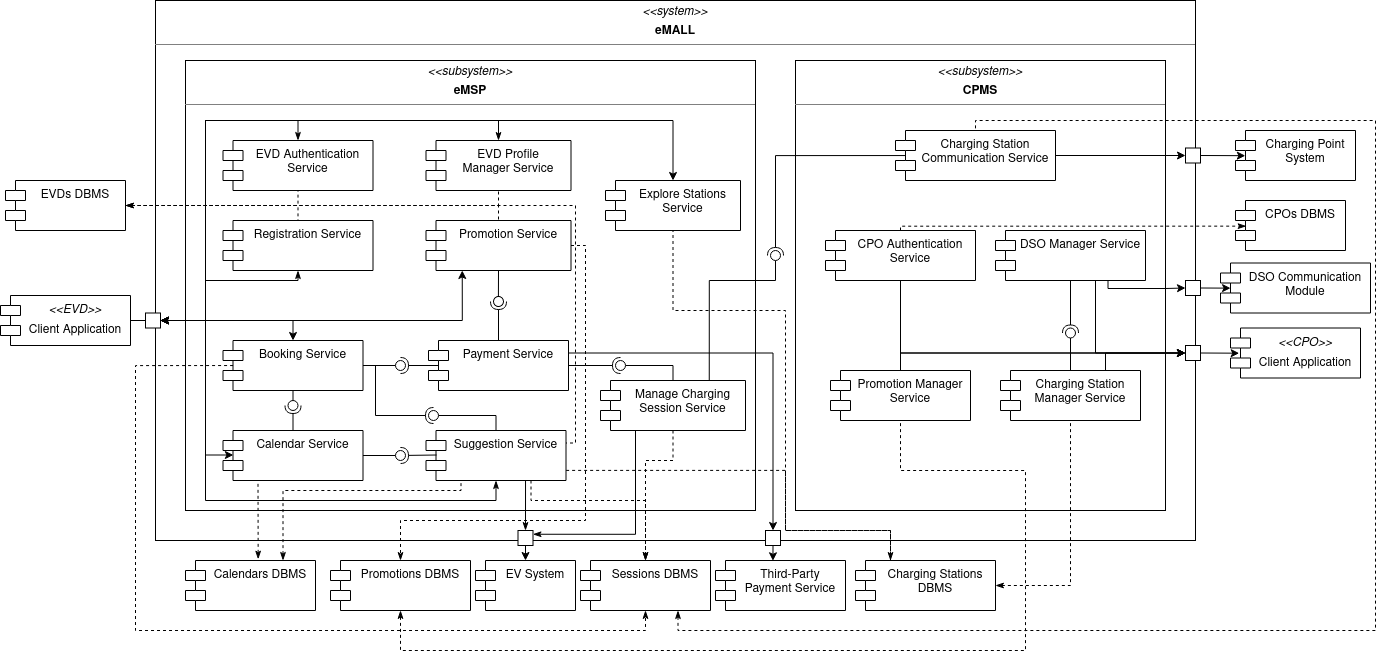
\includegraphics[width=1\linewidth]{ComponentDiagram/component_diagram}
        \caption{Component diagram of the eMALL system.}
        \label{fig: cd}
    \end{center}
\end{figure}


\section{Deployment View}
\label{sec: deployment_view}%
The following deployment diagram shows how all the components are distributed into different nodes,
highlighting how they communicate with each other. \\
The next paragraphs will go into details about the reasons behind the design choices. \\
The deployment diagram is:
\begin{figure} [H]
    \begin{center}
        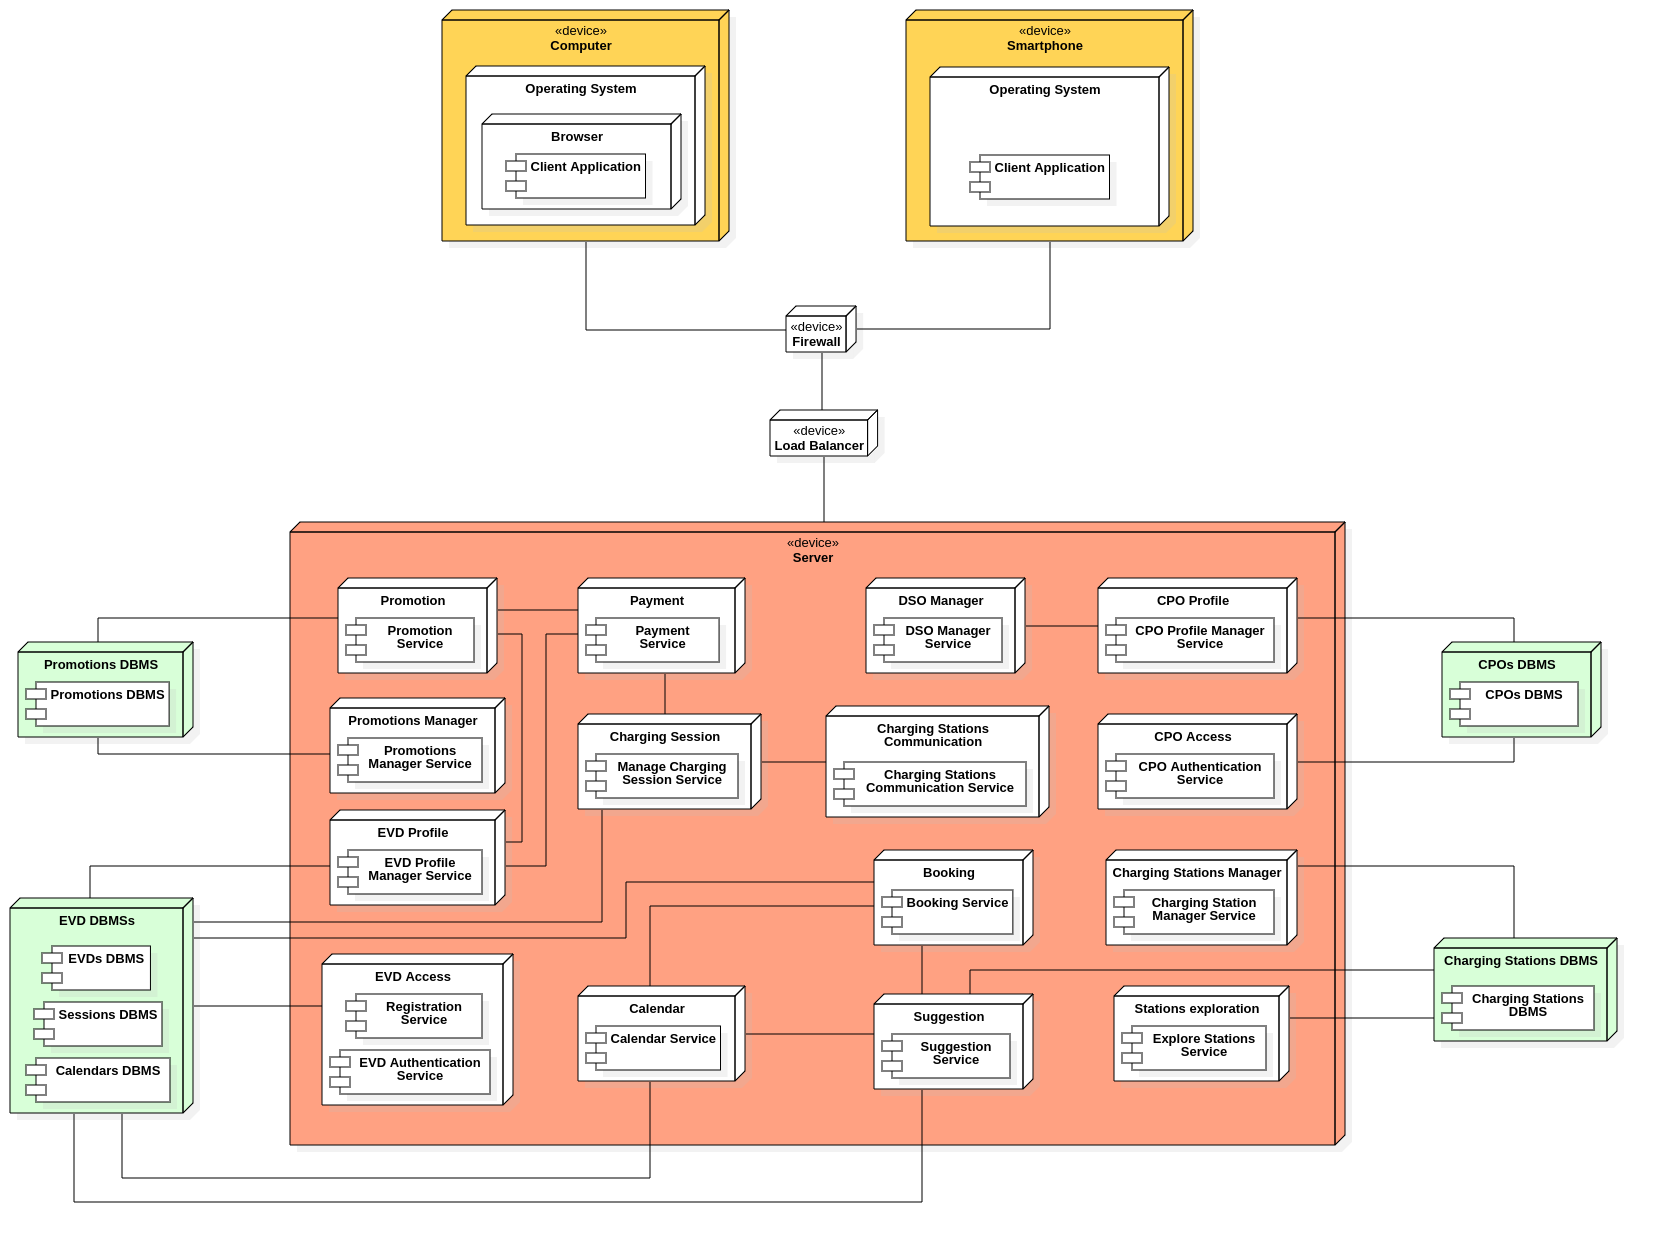
\includegraphics[width=1\linewidth]{DeploymentDiagram/deployment_diagram}
        \caption{Deployment diagram of the eMALL system.}
        \label{fig: depl_diagram}
    \end{center}
\end{figure}

\subsection{Connection to the server}
\label{subsec:connection_to_the_server}%
EVDs and CPOs can access the eMALL system from both PC and smartphones.
In the first case, it is necessary to use a browser to load the system's web page.
In the second case, the client will use the application after downloading it from the smartphone's store (Android or iOS).
When requests are sent to the server, first they pass into the firewall, so to avoid eventual cyberattacks on the system,
then they pass into the load balancer, so to optimize resource usage,
improve performance, and increase the availability of several services.
Requests are now ready to be handled by the eMALL services. \\
It follows the corresponding part from the deployment diagram:
\begin{figure} [H]
    \begin{center}
        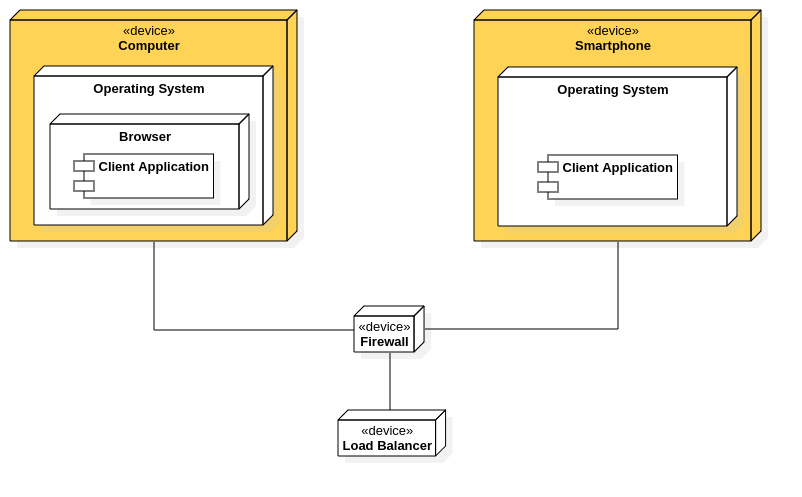
\includegraphics[width=0.7\linewidth]{DeploymentDiagram/connection}
        \caption{Connection to the server diagram.}
        \label{fig: connection}
    \end{center}
\end{figure}

\subsection{Promotions}
\label{subsec:promotions}%
Promotion DBMS is one of the four identified DBMS nodes.
The choice of dividing it from other DBMSs relies on the will to better scale the system.
In this way, it is easier to guarantee the availability of other services that don't work with promotions,
and maintenance sessions are facilitated too.
It has not been grouped with other DBMSs into the same node because Promotions DBMS is also used by CPOs,
so the system needs to guarantee a high level of scalability to assure business functionalities to the companies. \\
It follows the corresponding part from the deployment diagram:
\begin{figure} [H]
    \begin{center}
        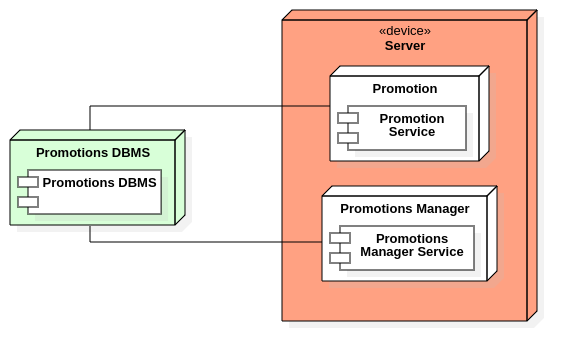
\includegraphics[width=0.6\linewidth]{DeploymentDiagram/promotion}
        \caption{Promotions managing diagram.}
        \label{fig: promotion}
    \end{center}
\end{figure}

\subsection{EVD interactions}
\label{subsec:evd_interactions}%
This section shows how the system communicates with \verb|EVDs DBMS|\@.
We choose to group \verb|EVDs DBMS|, \verb|Sessions DBMS|, and \verb|Calendars DBMS| into the same node because
they all receive requests from the services only in case of interactions with EVDs.
Considering that they don't introduce strict time response requirements,
it was not necessary to insert new physical nodes for the managing of the DBMSs. \\
It follows the corresponding part from the deployment diagram:
\begin{figure} [H]
    \begin{center}
        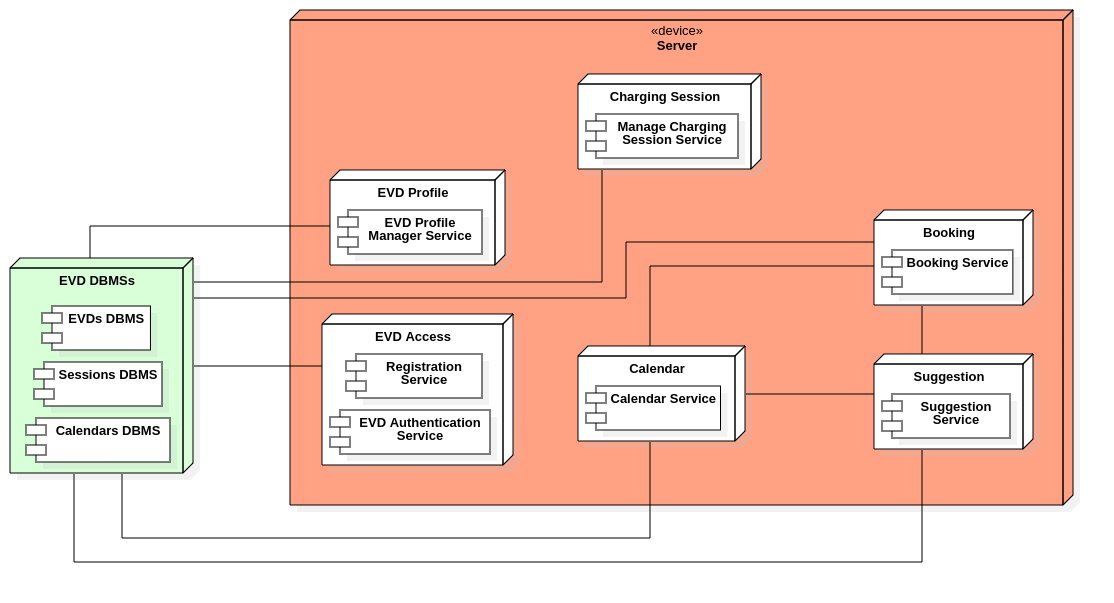
\includegraphics[width=\linewidth]{DeploymentDiagram/EVD_interactions}
        \caption{EVD interactions diagram.}
        \label{fig: evd_interactions}
    \end{center}
\end{figure}

\subsection{CPOs DBMS}
\label{subsec:cpo_dbms}%
The components that communicate with the CPOs DBMS are the Authentication Service and the CPO Profile Manager Service.
When another service needs to get or to update information about a CPO, the request is handled by the CPO Profile node.
The DBMS is used by CPOs, so it is deployed in a single node to better scale the system,
and to guarantee business functionalities to the companies. \\
It follows the corresponding part from the deployment diagram:
\begin{figure} [H]
    \begin{center}
        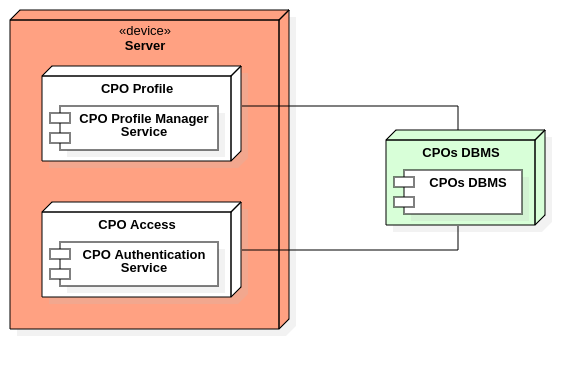
\includegraphics[width=0.6\linewidth]{DeploymentDiagram/CPO_DBMS}
        \caption{CPOs DBMS managing diagram.}
        \label{fig: cpo_dbms}
    \end{center}
\end{figure}

\subsection{Charging stations communication}
\label{subsec:charging_stations_communication}%
Suggestion and Stations exploration nodes read from the DBMS
to get the position of the stations that will be elaborated or shown to the user.
Charging Station Manager Service can also write or update the instances of the DBMS\@.
The DBMS is used by CPOs, so it is deployed in a single node to better scale the system,
and to guarantee business functionalities to the companies. \\
It follows the corresponding part from the deployment diagram:
\begin{figure} [H]
    \begin{center}
        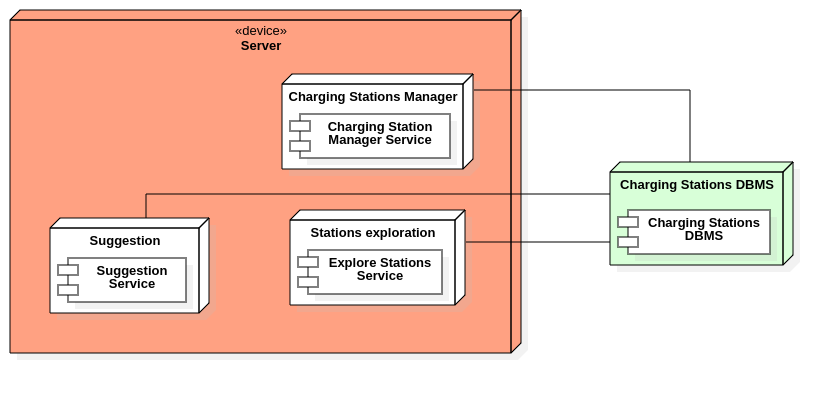
\includegraphics[width=0.85\linewidth]{DeploymentDiagram/charging_stations_communication}
        \caption{Charging stations communication diagram.}
        \label{fig: charing_stations_dbms}
    \end{center}
\end{figure}

\subsection{Services}
\label{subsec:services}%
The section shows all the identified nodes in which services run. \\
Decisions have been made giving particular attention to the concepts of loose coupling and high cohesion.
As explained in Sam Newman's \textit{Building Microservices}, they are defined as follows:
\begin{itemize}
    \item \textbf{Loose coupling.} \textit{When services are loosely coupled, a change to one service should not require a change to another.
    The whole point of a microservice is being able to make a change to one service  and deploy it,
        without needing to change any other part of the system.}
    \item \textbf{High Cohesion.} \textit{We want related behavior to sit together, and unrelated behavior to sit elsewhere.
    Making changes in lots of different places is slower, and deploying lots of services at once is risky, both of which we want to avoid.}
\end{itemize}
The following image wants also to highlight the relations between different services, which are direct consequences of the
communication interfaces previously shown in the component diagram.
\begin{figure} [H]
    \begin{center}
        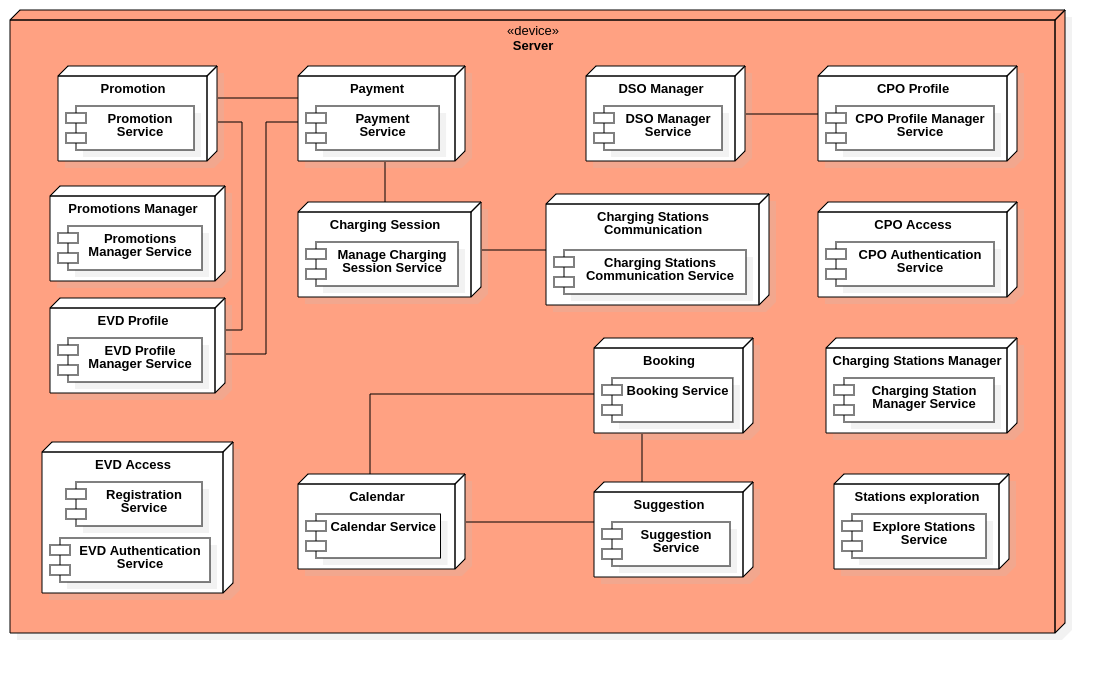
\includegraphics[width=\linewidth]{DeploymentDiagram/server}
        \caption{Server services diagram.}
        \label{fig: services}
    \end{center}
\end{figure}



\section{Runtime View}
\label{sec: runtime_view}%


\section{Component Interfaces}
\label{sec: component_interfaces}%


\section{Selected Architectural Styles and Patterns}
\label{sec: patterns}%


\section{Other Design Decisions}
\label{sec: other_design_decisions}%
